\documentclass[11pt,letter]{article}
\usepackage[top=1.00in, bottom=1.0in, left=1.1in, right=1.1in]{geometry}
\renewcommand{\baselinestretch}{1}
\usepackage{graphicx}
\usepackage{natbib}
\usepackage{amsmath}
\usepackage{hyperref}

\def\labelitemi{--}
\parindent=0pt
\parskip=5pt

\begin{document}
\bibliographystyle{/Users/Lizzie/Documents/EndnoteRelated/Bibtex/styles/besjournals}
\renewcommand{\refname}{\CHead{}}

\title{Comparing \emph{Quercus} model from \\ Duputie vs. van der Meersch}
\author{Lizzie, Isabelle Chuine, Ben Cook, Victor van der Meersch}
\date{\today}
\maketitle

\section*{Overview}
For the mean results for \emph{Quercus} we wondered whether the Leaf model parameterization was driving the results. It's currently set to have a -4.5 maximum temperature. To check this we created an updated file (\verb|Quercus_robur_ADuputie_updated23June2023.species|) using the leaf model parameterization from Van der Meersch \& Chuine 2023 (\verb|cmaes_fit_subset2_rep2.species|). After reviewing the results, Victor replied:

\begin{quote}
I am surprised by the fitness with the updated parameters, which seems veeery low, though there are Quercus indivuals in these latitude.
Maybe it is because we only extracted the leaf/flower parameters from the inverse calibration set?
If it is not time consuming, you could try to run simulations directly with the "cmaes\_fit\_subset2\_rep2.species" file, even though extra precautions must be taken when analysing the results.
\end{quote}

And Isabelle agreed so now I ran with the new parameter set. Below is a comparison of the results between the FULL updated parameters and Duputie (se Fig. \ref{fig:fruitmatdate}) which now clearly gets laters at higher latitudes, and matters to fitness (whereas before neither of these things happened). 

\section*{Based on historical climate}

See bottom panels of Fig. \ref{fig:histdup}-\ref{fig:histdnew}, trends are similar (MaturationIndex dominates fitness) but now fitness is now low as of latitudes 41 and 44 and higher. I was also struck by how the FruitMatDate changed, 

\begin{figure}[h!]
 \begin{center}
\noindent 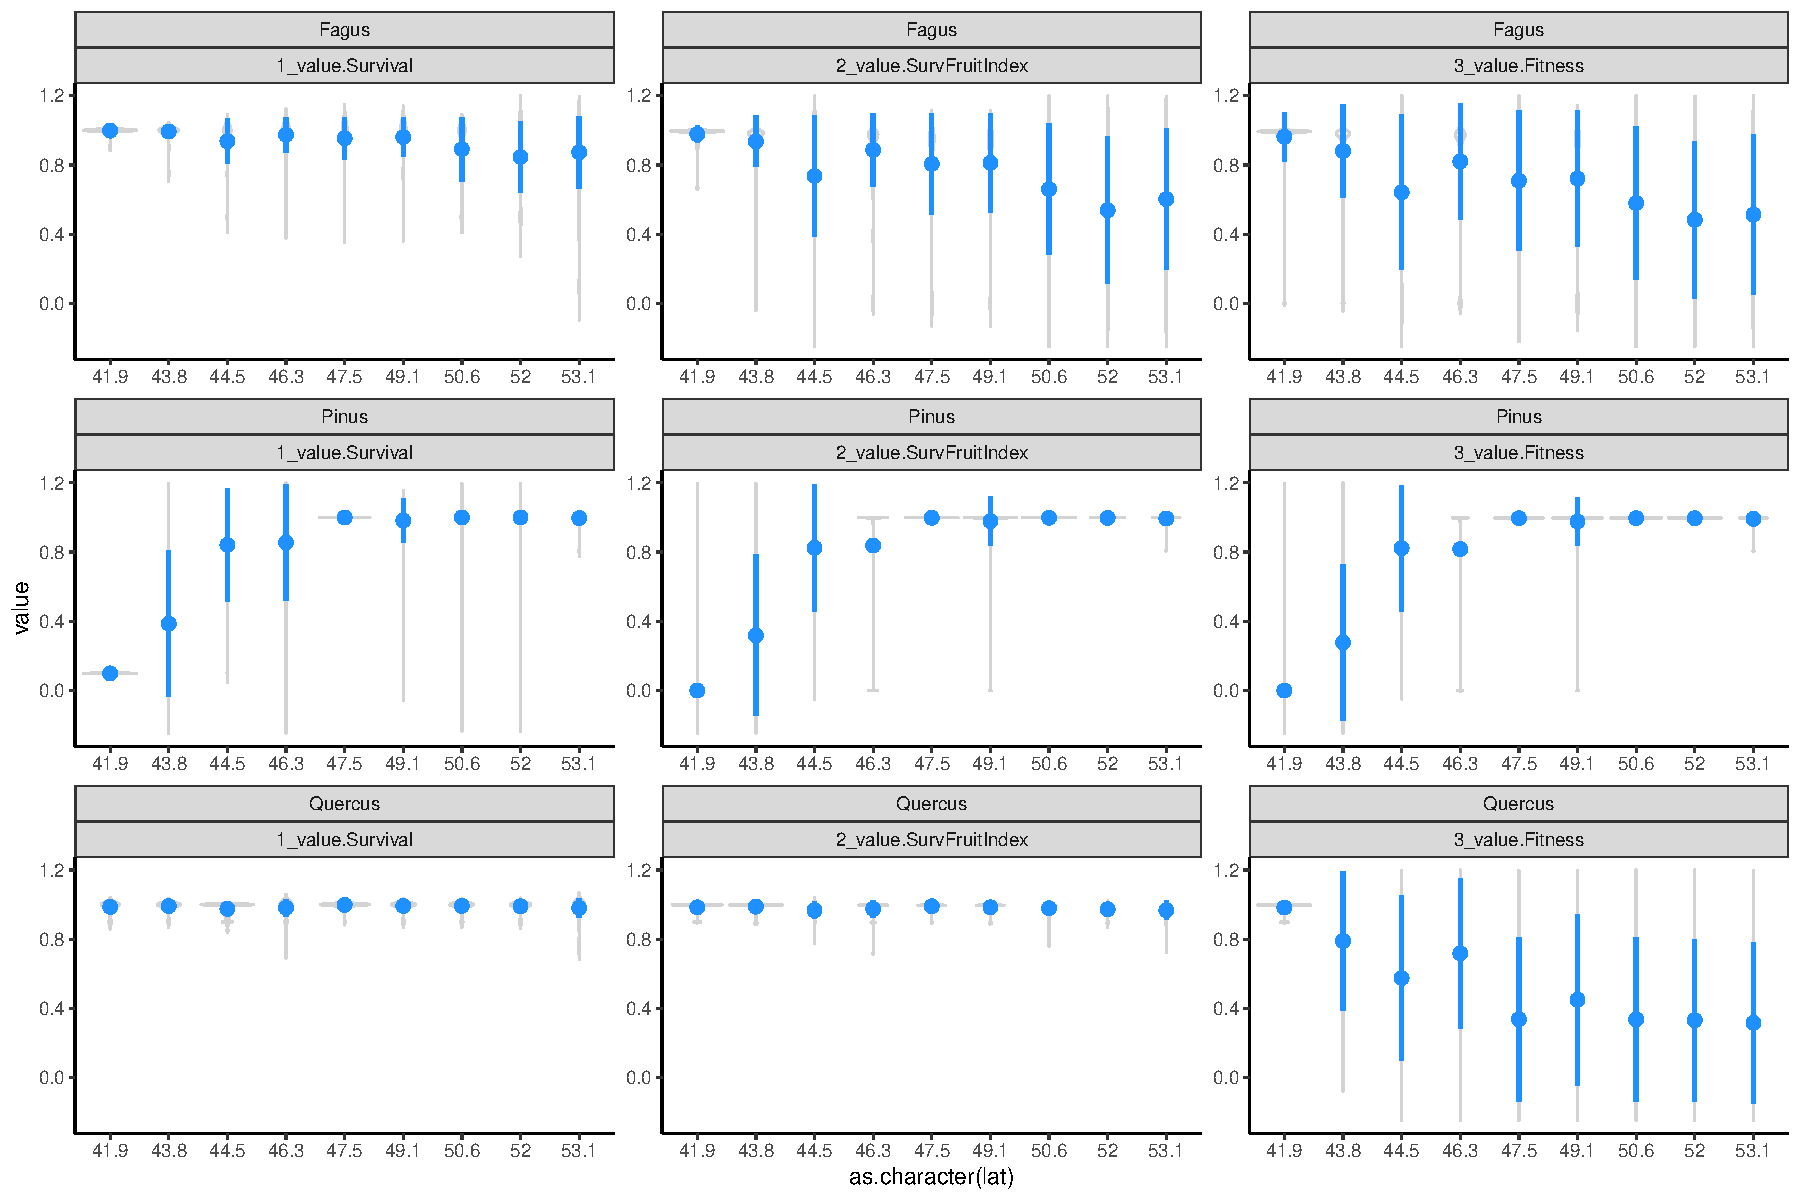
\includegraphics[width=1\textwidth]{..//analyses/graphs/phenofit/historical/fitnessBuildup_DuputieQuercus.pdf}
  \caption{\emph{Quercus} fitness across latitude (historical climate data) based on Duputie parameters. You can see PHENOFIT4 output at \url{https://github.com/lizzieinvancouver/climatehazards/tree/main/analyses/input/phenofit/querob_19512020_Duputie}.}
  \label{fig:histdup}
  \end{center}
\end{figure}

\begin{figure}[h!]
 \begin{center}
\noindent 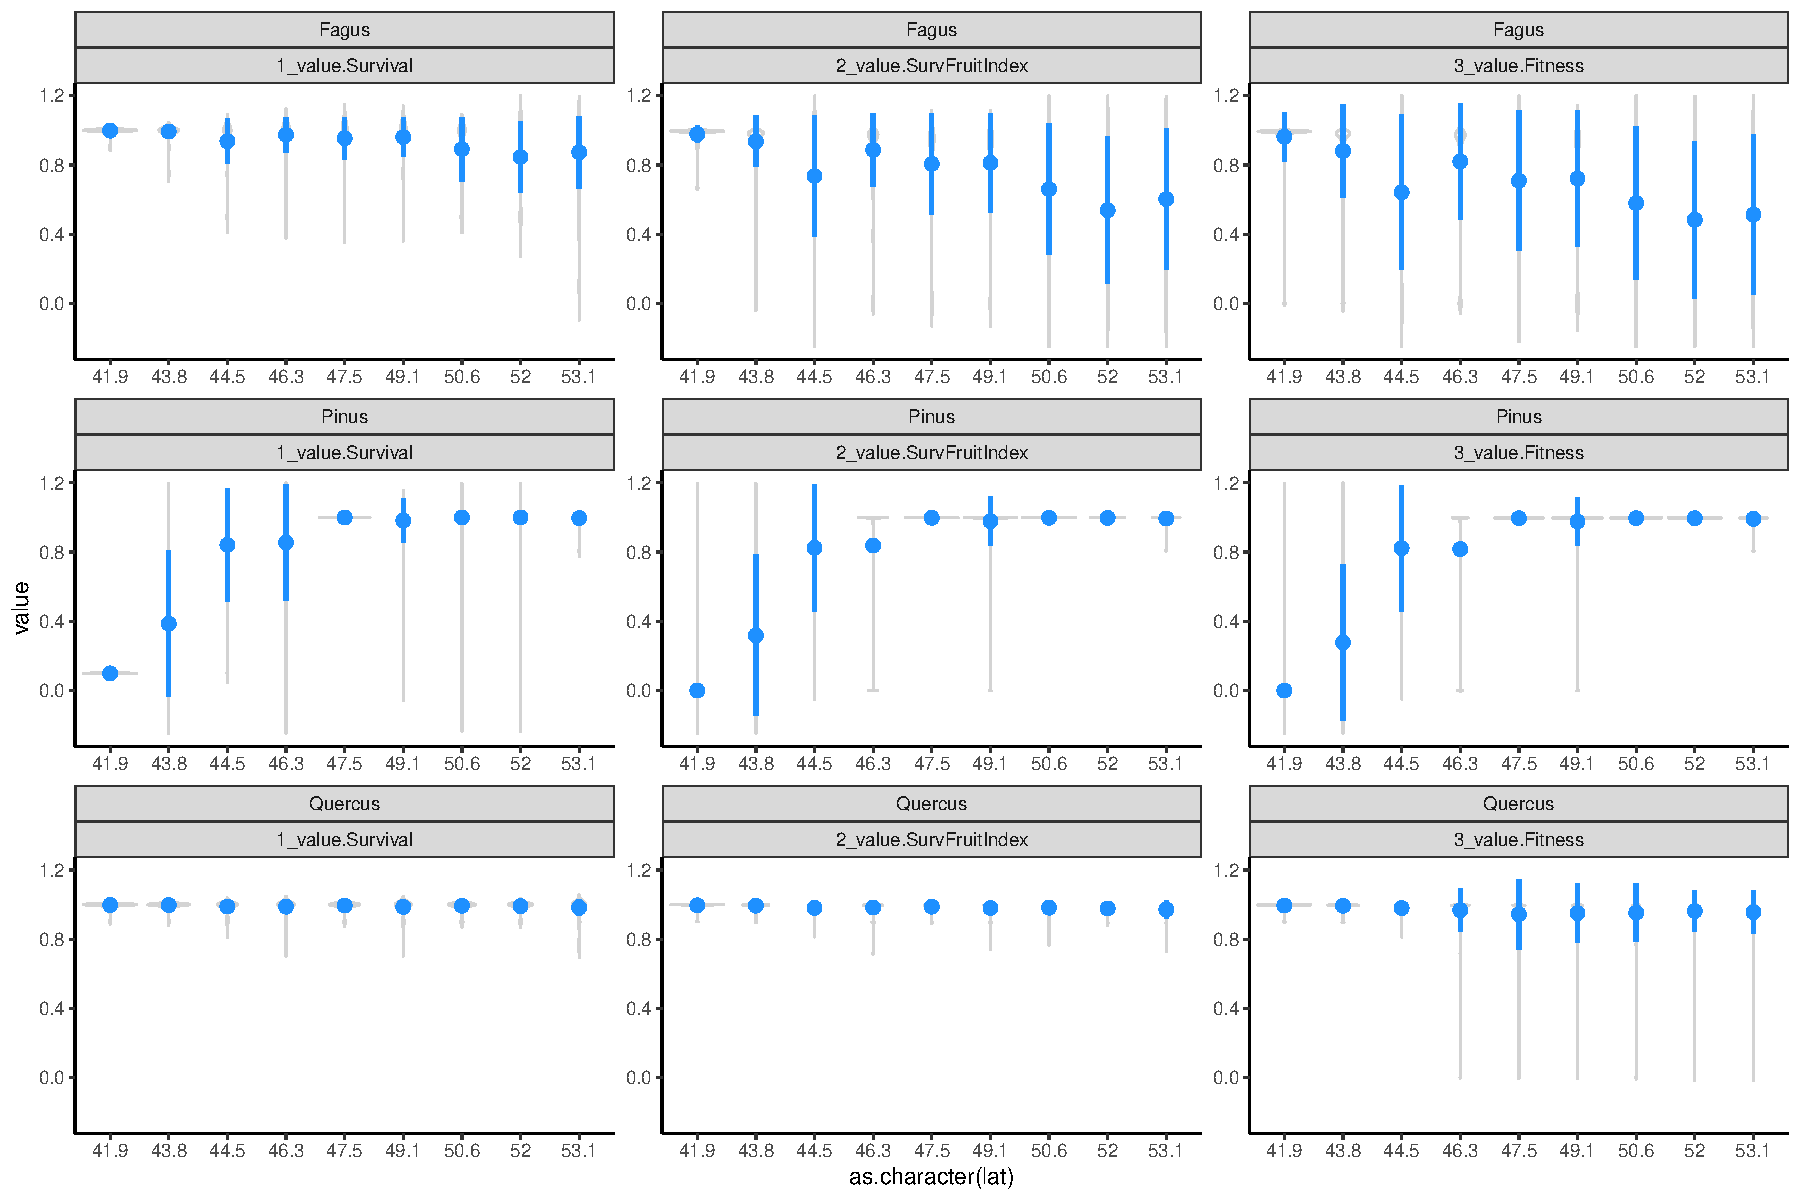
\includegraphics[width=1\textwidth]{..//analyses/graphs/phenofit/historical/fitnessBuildup.pdf}
  \caption{\emph{Quercus} fitness across latitude (historical climate data) based on updated ALL model parameters. You can see PHENOFIT4 output at \url{https://github.com/lizzieinvancouver/climatehazards/tree/main/analyses/input/phenofit/querob_19512020}.}
  \label{fig:histdnew}
  \end{center}
\end{figure}


\begin{figure}[h!]
 \begin{center}
\noindent 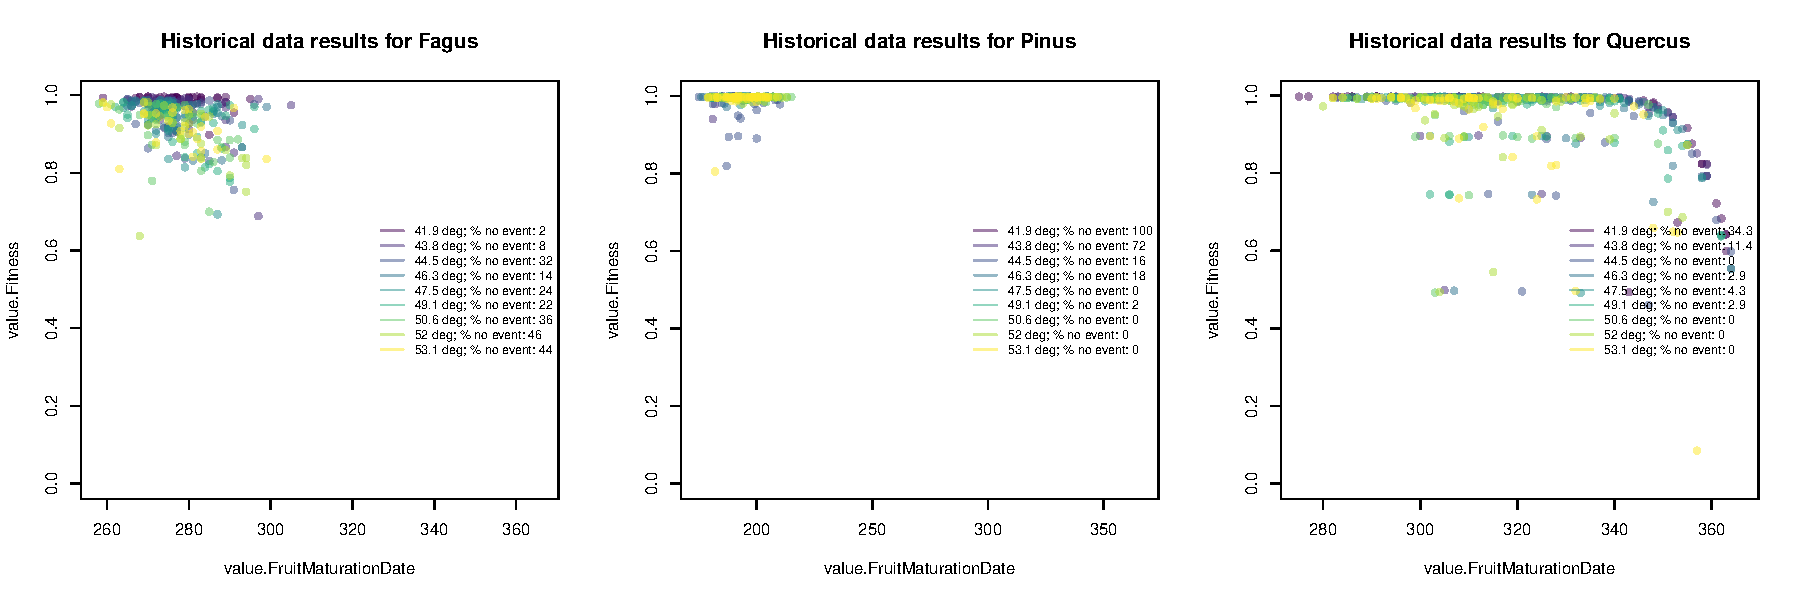
\includegraphics[width=1\textwidth]{..//analyses/graphs/phenofit/historical/allspp_xypoints_wprint_fruitmatdate_vsfitness.pdf}
  \caption{\emph{Quercus} fitness as a function of FruitMaturationDate (historical climate data) based on updated ALL model parameters. You can see the previous plot using the Duputie parameters at \url{https://github.com/lizzieinvancouver/climatehazards/blob/faaca3adcab9bf8d615732abf1ebfe00a1d52370/analyses/graphs/phenofit/historical/allspp_xypoints_wprint_fruitmatdate_vsfitness.pdf}.}
  \label{fig:fruitmatdate}
  \end{center}
\end{figure}


\clearall
\section*{Based on simulated climate with mean warming}

See Fig. \ref{fig:simsmeanDup}-\ref{fig:simsmeanUp}. Fitness is again affected mostly by MaturationIndex, and low at high warming.

\begin{figure}[h!]
 \begin{center}
\noindent 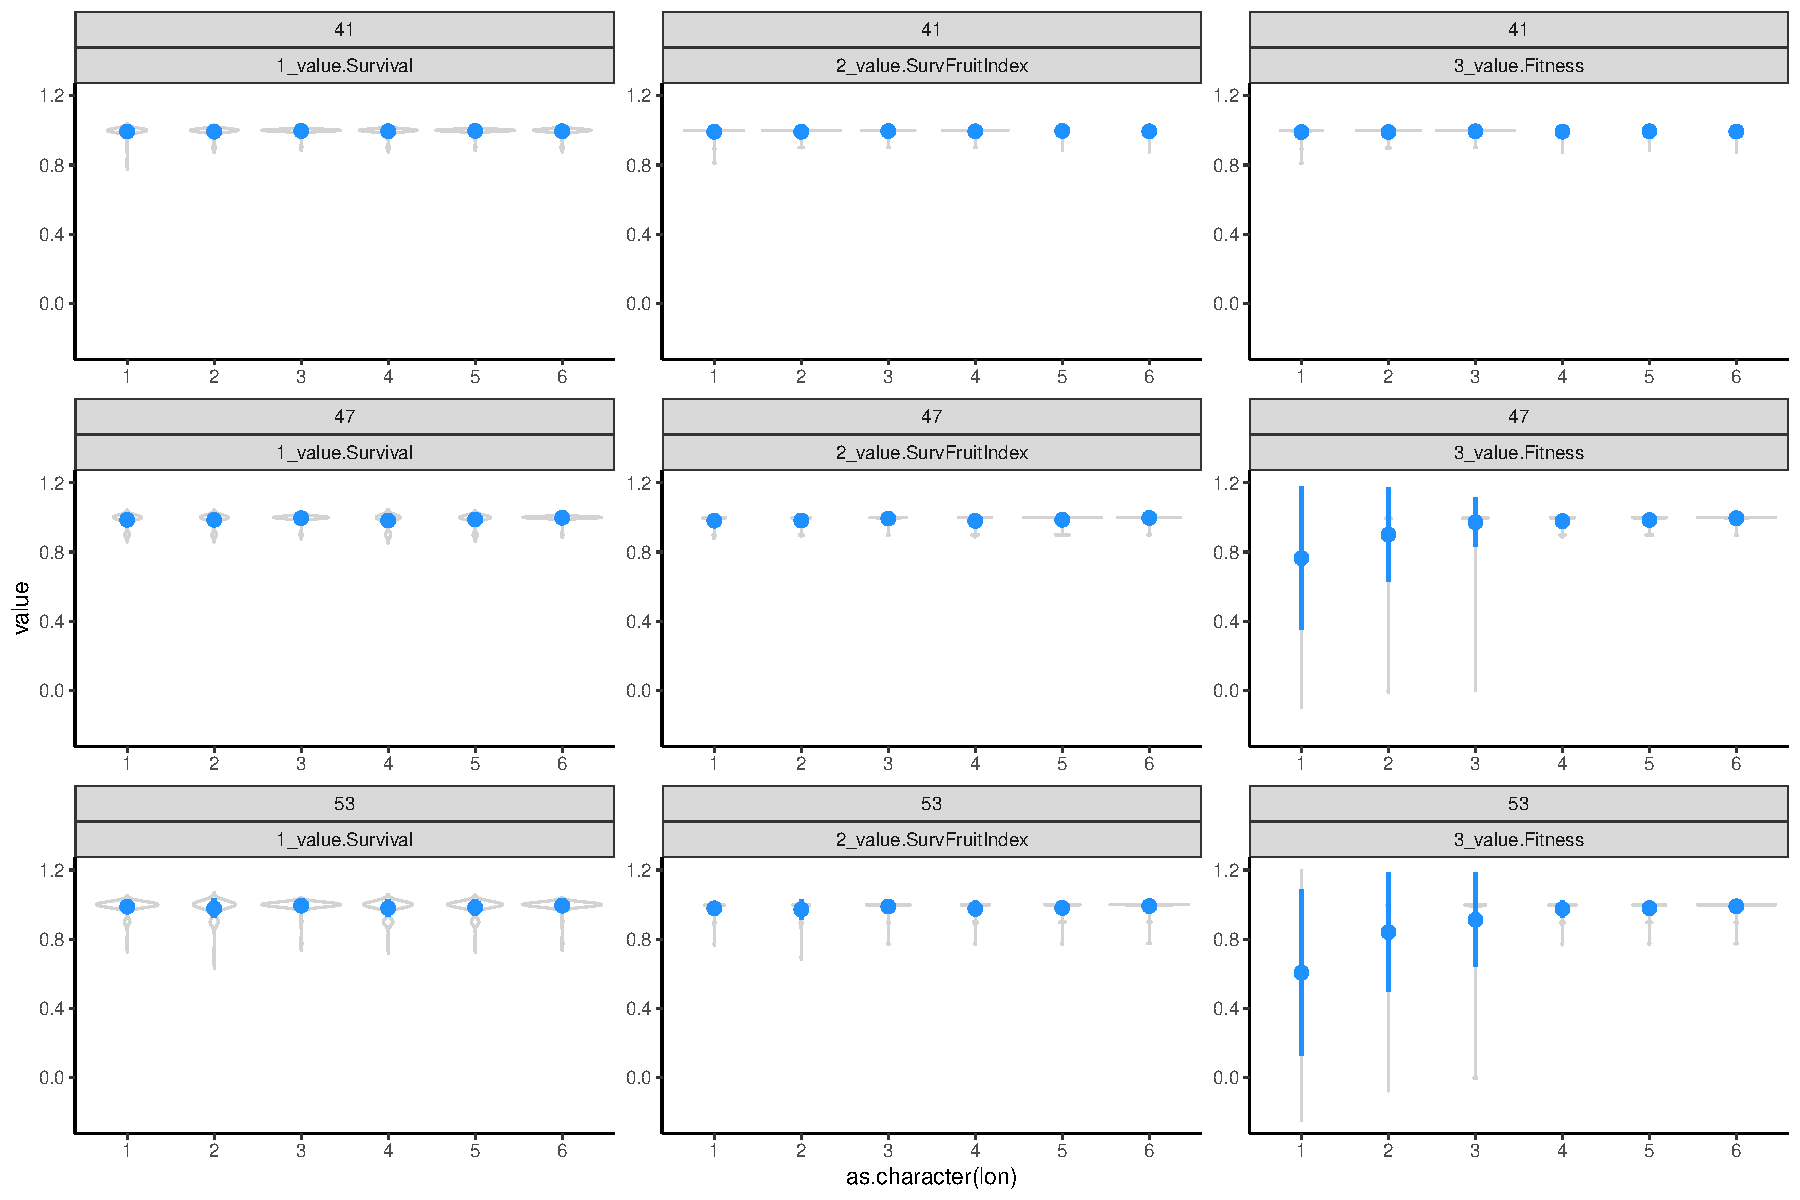
\includegraphics[width=1\textwidth]{..//analyses/graphs/phenofit/sims/querob_Duputie/meansim_3metricsQR.pdf}
  \caption{\emph{Quercus} across 0 (1) to $+$5 (6) mean warming, based on Duputie parameters. To see the underlying components of the model, look for `meansim' QR files at \url{https://github.com/lizzieinvancouver/climatehazards/tree/main/analyses/graphs/phenofit/sims/querob_Duputie}.}
  \label{fig:simsmeanDup}
  \end{center}
\end{figure}

\begin{figure}[h!]
 \begin{center}
\noindent 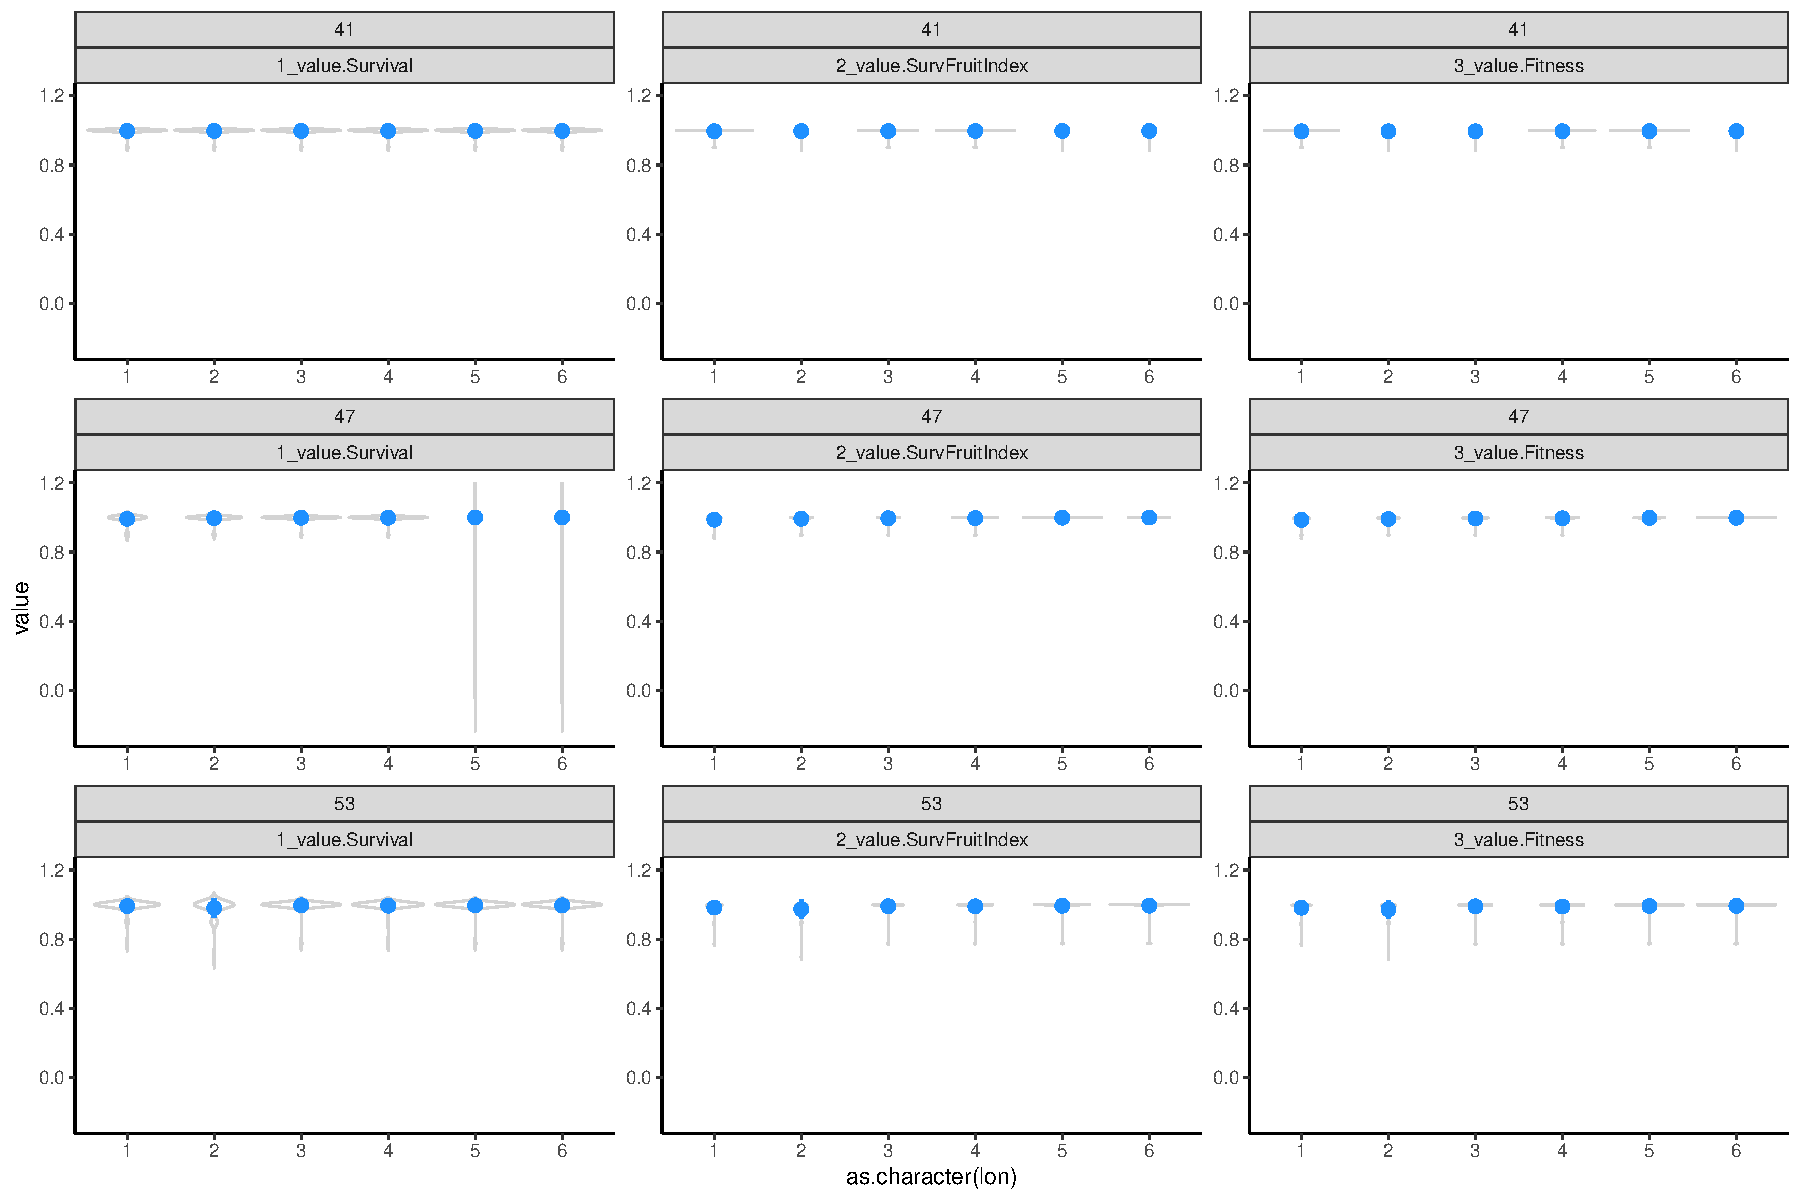
\includegraphics[width=1\textwidth]{..//analyses/graphs/phenofit/sims/metrics3/meansim_3metricsQR.pdf}
  \caption{\emph{Quercus} across 0 (1) to $+$5 (6) mean warming, based on updated parameters. To see the underlying components of the model, look for `meansim' QR files in \url{https://github.com/lizzieinvancouver/climatehazards/tree/main/analyses/graphs/phenofit/sims}}
  \label{fig:simsmeanUp}
  \end{center}
\end{figure}


\clearall
\section*{Based on simulated climate with changing variance}

See Fig. \ref{fig:simssdDup}-\ref{fig:simssdUp}. Fitness dominated by FruitIndex (I think) and decreasing with increasing variance.
\begin{figure}[h!]
 \begin{center}
\noindent \includegraphics[width=1\textwidth]{..//analyses/graphs/phenofit/sims/querob_Duputie/sdsim_3metricsQR.pdf}
  \caption{\emph{Quercus} across changing variance, based on Duputie parameters. To see the underlying components of the model, look for `dssim' QR files at \url{https://github.com/lizzieinvancouver/climatehazards/tree/main/analyses/graphs/phenofit/sims/querob_Duputie}.}
  \label{fig:simssdDup}
  \end{center}
\end{figure}

\begin{figure}[h!]
 \begin{center}
\noindent \includegraphics[width=1\textwidth]{..//analyses/graphs/phenofit/sims/metrics3/sdsim_3metricsQR.pdf}
  \caption{\emph{Quercus} across changing variance, based on updated parameters. To see the underlying components of the model, look for `sdsim' QR files in \url{https://github.com/lizzieinvancouver/climatehazards/tree/main/analyses/graphs/phenofit/sims}}
  \label{fig:simssdUp}
  \end{center}
\end{figure}



\end{document}
